\section{Bibliography Review}
\label{sec:bibliography-review}

A bibliographical search was performed to determine th current state-of-the-art in market-making research using reinforcement learning.
The analysis performed showed a gap in the literature regarding simulations with varying market regimes and non-stationary environments,
which we aim to address in our research.
We determined the best performing algorithms and state-action spaces used in the literature,
and the most common data types and reward structures used in the references.
The search was made using the Web of Science repository, covering the last 5 years, with the following search key:

\small
\begin{verbatim}
(
    "reinforcement learning" OR
    "optimal control" OR
    "control theory" OR "machine learning"
)
AND
(
    "market making" OR "market maker"
)
\end{verbatim}

Initially, 59 references were selected and deemed relevant to the project,
with 23 of them being effectively used in our analysis, and 5 additional references being added to the list after the initial selection.

\subsection{Data Type}
\label{subsec:data-type}
The majority of the references used historical data, while the second most common type was agent-based simulations,
where generative agents are trained against observed market messages and used to simulate the LOB environment~\cite{Frey2023, Ganesh2019}
trading off control over the market dynamics for replicating observed market flow.

\begin{figure}
    \centering
    \includegraphics[width=0.9\columnwidth]{images/data}
    \caption{Data types used in the references.}
    \label{fig:figure7}
\end{figure}

The third most common were stationary processes including Geometric Brownian Motion and Poisson processes~\cite{Gasperov2021, Sun2022} for
order arrival and price dynamics, while some used the Hawkes process for simulating order arrival times~\cite{Jerome2022, Selser2021}.
Overall, the references shown in \autoref{fig:figure7} demonstrate a preference for historical data and model-based simulators,
and although being extremely promising approaches, neither completely account for changing market regimes and scenarios where impact and
slippage have a more prominent effect on the agent's performance.
With no references using both simulated data and reinforcement learning agents instead of closed-form solutions,
we aim to address this gap in the literature by implementing a reinforcement learning agent and testing its robustness and generalization capabilities under non-stationary environments.

\subsection{State, Action, and Reward Spaces}
\label{subsec:spaces}

Most analyzed references defined state spaces primarily based on market-level observations, as shown in \autoref{fig:state}.
specifically top-of-book quotes and N-depth book levels which align well with the real-time data available to market-making agents~\cite{He2023, Bakshaev2020}.
Additionally, agent inventory was also a common feature, reflecting the importance of managing risk and liquidity in market-making strategies~\cite{Patel2018, Ganesh2019}.
The tagged action spaces was mostly made up only one pair of quotes, with some references allowing the choice of multiple bid-ask levels.
Some references also used book levels as discrete action space variables, displayed in \autoref{fig:action}.

Finally, almost all reward structures, shown in \autoref{fig:reward},
were based on intraday or daily profit-and-loss scores, with either running liquidation, inventory penalties, or a combination of both.
The tagged action space variables also includes a separate ``Inventory'' variable that refers to portfolio strategies that output a target maximum inventory.
For implementations that use specific quantities per order, no additional tags were used,
as only 1 reference did not add quantities as part of the action space and instead used fixed quantities.

\begin{figure}
    \centering
    % First row: Two side-by-side subfigures
    \begin{subfigure}{.9\columnwidth}
        \centering
        \includegraphics[width=\linewidth]{images/reward_space}
        \caption{Tagged reward space function variables}
        \label{fig:reward}
    \end{subfigure}
    \vspace{0.5em}
    \begin{subfigure}{.9\columnwidth}
        \centering
        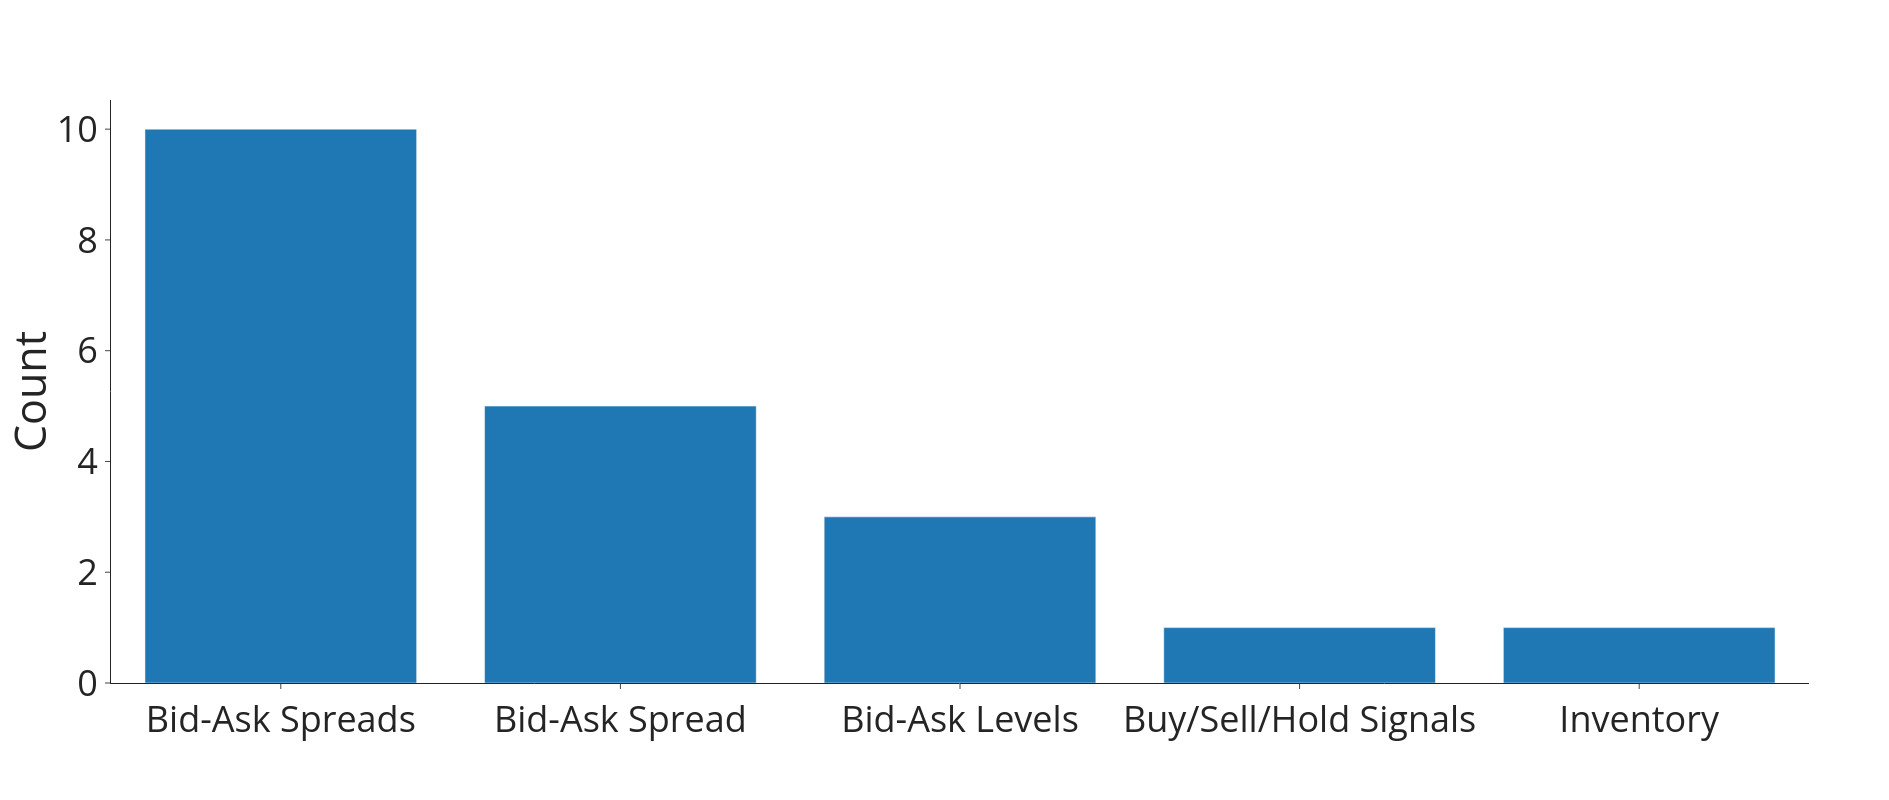
\includegraphics[width=\linewidth]{images/action_space}
        \caption{Tagged action space variables}
        \label{fig:action}
    \end{subfigure}
    \vspace{0.5em} % Adjust vertical spacing
    \begin{subfigure}{.9\columnwidth}
        \centering
        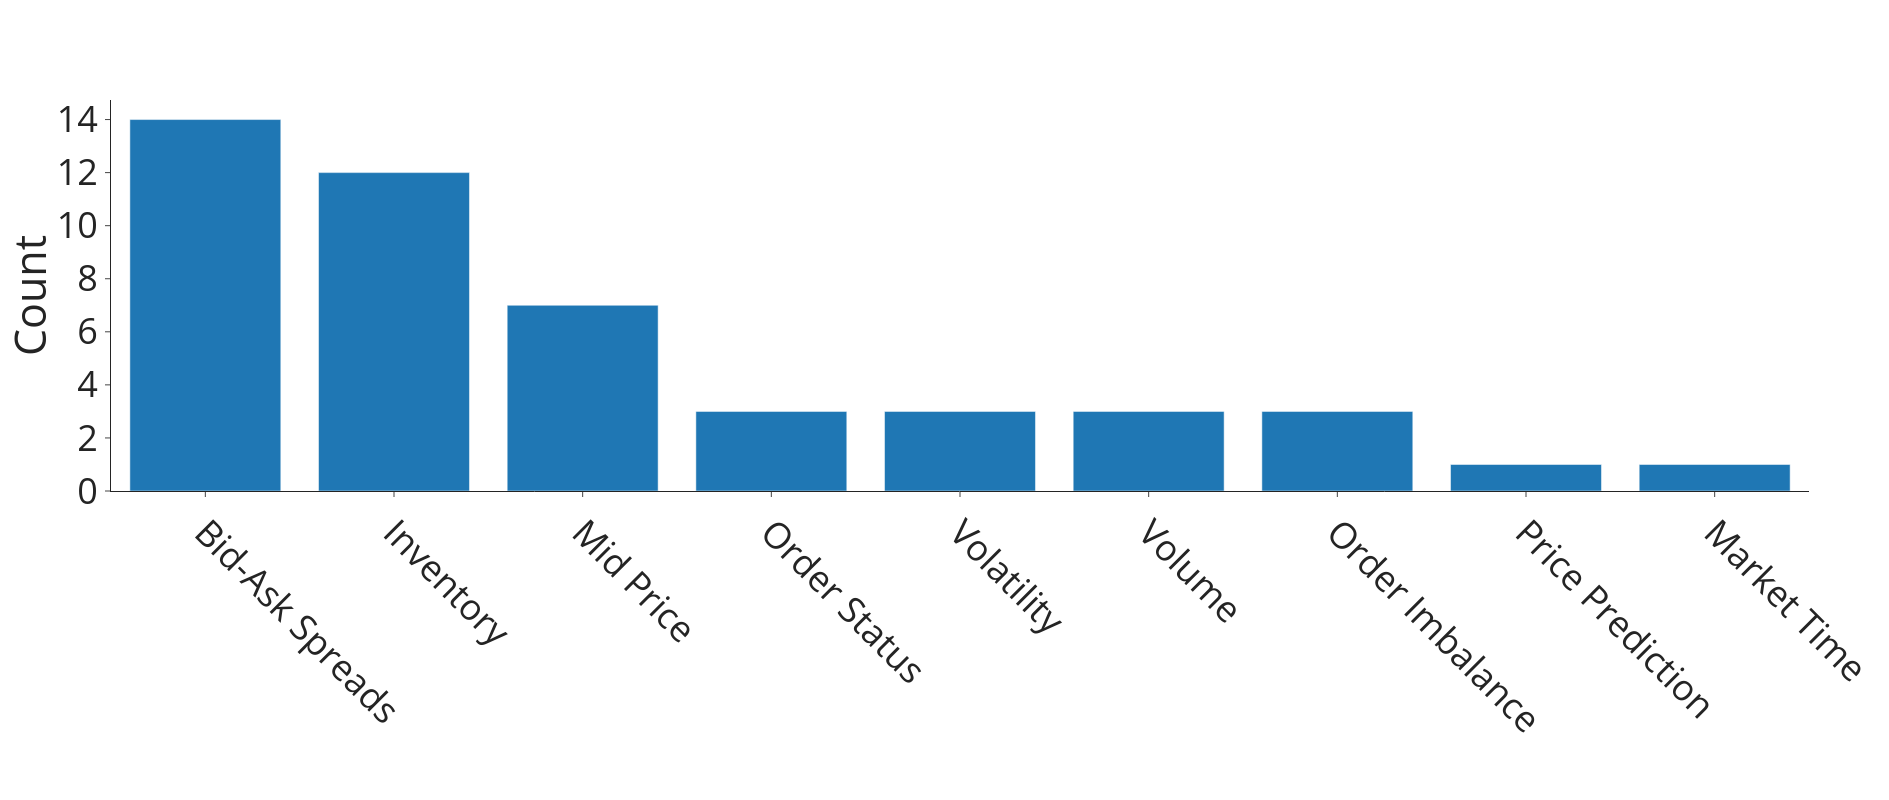
\includegraphics[width=\linewidth]{images/state_space}
        \caption{Tagged state space variables}
        \label{fig:state}
    \end{subfigure}
\end{figure}

\subsection{Chosen Algorithms}
\label{subsec:chosen-algorithms}
Most references used Deep Q-Learning and Actor-Critic methods, leveraging neural networks for the optimal policy or state-value function estimation,
due to the high-dimensional nature of limit order books~\cite{Patel2018, Ganesh2019}.
The most used algorithms were PPO and DQN, as shown in \autoref{tab:table1},
both being the best performers in terms of convergence and generalization capabilities in the literature~\cite{Sun2022, Gasperov2021a}, with some references using DDQN variants.
The literature on model-free approaches overall demonstrated strong adaptability capabilities towards changing market conditions
while still maintaining acceptable training times.
Overall, the performed bibliographical review underscores the growing relevance and preference for reinforcement learning algorithms in the market-making domain,
particularly when combined with realistic spatial and temporal state representations.

% table:
\begin{table}
    \centering
    \begin{tabular}{|c|c|}
        \hline
        \textbf{Algorithm}           & \textbf{References} \\
        \hline
        Closed-Form Expression       & 8                   \\
        Deep (Double) Q-Learning     & 6                   \\
        Proximal Policy Optimization & 2                   \\
        Q-Learning                   & 2                   \\
        SARSA                        & 1                   \\
        Vanilla Policy Gradient      & 1                   \\
        SAC                          & 1                   \\
        \hline
    \end{tabular}
    \caption{Algorithms used in the references.}
    \label{tab:table1}
\end{table}
